\documentclass[12pt,a4paper]{article}
\usepackage{kotex}
\usepackage{hyperref}
\usepackage{amssymb}
\usepackage{amsmath,amsthm,amsfonts,amscd}
\usepackage[utf8]{inputenc}
\usepackage{geometry}
\usepackage{titling}
\usepackage{titlesec}
\usepackage{xcolor}
\usepackage{graphicx}
\usepackage{fancyhdr}
\usepackage{lipsum} % for generating sample text
\usepackage{wallpaper}
\usepackage{tabularx}
\usepackage{booktabs}
\usepackage{setspace}
\usepackage{tikz}
%\usepackage{pgf-pie}

% Define custom colors
\definecolor{darkblue}{RGB}{25,25,112}  % Midnight Blue
\definecolor{lightblue}{RGB}{173,216,230}  % Light Blue

\usepackage{geometry}
\geometry{a4paper,left=.7in,right=.7in,top=1in,bottom=1in,heightrounded}
% Header and Footer
\pagestyle{fancy}
\fancyhead{}
\fancyhead[L]{\textcolor{darkblue}{\bf P.A.N.D.A's PUBAO: Discrete Logarithm Calculator Development}}
\fancyfoot{}
\fancyfoot[C]{\thepage}
\renewcommand{\headrulewidth}{0.5pt}
\renewcommand{\footrulewidth}{0.5pt}
\renewcommand{\headrule}{\hbox to\headwidth{\color{lightblue}\leaders\hrule height \headrulewidth\hfill}}
\renewcommand{\footrule}{\hbox to\headwidth{\color{lightblue}\leaders\hrule height \footrulewidth\hfill}}

% Title Styling
\pretitle{\begin{center}\Huge\color{darkblue}\bfseries\scshape}
	\posttitle{\end{center}\vskip 0.5em}
\preauthor{\begin{center}\large\color{lightblue!50!black}\scshape\lineskip 0.5em}
	\postauthor{\end{center}}
\predate{\begin{center}\color{darkblue}\large\scshape}
	\postdate{\end{center}}

% Section Styling
\titleformat{\section}
{\color{darkblue}\normalfont\Large\bfseries\scshape}
{\color{darkblue}\thesection}{1em}{}
\titleformat{\subsection}
{\color{lightblue!50!black}\normalfont\large\bfseries\scshape}
{\color{lightblue!50!black}\thesubsection}{1em}{}

%Tcolorbox
\usepackage[most]{tcolorbox}
\tcbset{colback=white, arc=5pt}

% Font Selection
\renewcommand*\familydefault{\sfdefault} 

% Background Image
%\ULCornerWallPaper{1}{panda3.png} % Replace 'background.jpg' with your image file 

% Title, Author, Date
\title{P.A.N.D.A's PUBAO: \\Discrete Logarithm Calculator Development}
\author{\textcolor{lightblue!50!black}{\bf 지용현, 김예찬, 문예찬, 유근오}}
\date{\today}
\setstretch{1.5}
\begin{document}
	
	\maketitle
	\thispagestyle{empty}  % Removes header/footer on first page
	\begin{figure}[h!]
		\centering
		\includegraphics[scale=.5]{panda4.png}
	\end{figure}
	\newpage  % Ensures that content starts on the second page
	
	\tableofcontents
	\newpage
	\section{Team Overview}
	\begin{itemize}
		\item \textbf{Team Name:} \textcolor{magenta}{\bf P.A.N.D.A. 
		\text{\small(Programmers Aspiring to Navigate Digital Arithmetic)} }
		\item \textbf{Project Name:} \textcolor{magenta}{\bf PUBAO \text{\small(P.A.N.D.A.'s Unbounded Big Arithmetic Operations)}}
		\item \textbf{Member:}
		\begin{itemize}
			\item[$\blacktriangleright$] \textcolor{darkblue}{\bf 지용현 (Leader)}
			\begin{itemize}
				\item[-] \textbf{Strategic Planning:} 프로젝트의 전반적인 방향을 설정하고 목표과 목적이 프로젝트 비전을 이끌어 나간다.
				\item[-] \textbf{Algorithm Implementation:} 계산 알고리즘의 실제 구현과 더불어 라이브러리와의 원활한 통합을 진행한다.
			\end{itemize}
		\vspace{8pt}
		\item[$\blacktriangleright$] \textcolor{darkblue}{\bf 김예찬 (Validator) }
		\begin{itemize}
			\item[-] \textbf{Quality Assurance:} 개발된 모듈이 버그가 없는지 확인한다.
			\item[-] \textbf{Feedback Loop:} 사용자 피드백을 수집하고 지속적인 개선을 촉진한다.
		\end{itemize}
	\vspace{8pt}
			\item[$\blacktriangleright$] \textcolor{darkblue}{\bf 문예찬 (Builder)}
		\begin{itemize}
			\item[-] \textbf{Core Development:} 필수 모듈 개발을 주도하고, 성능이 프로젝트 요구 사항에 부합하는지 확인한다.
			\item[-] \textbf{Integration:} 큰 정수 연산 라이브러리를 계산기와 통합하여 원활하고 오류 없는 작동을 보장한다.
		\end{itemize}
	\vspace{8pt}
			\item[$\blacktriangleright$] \textcolor{darkblue}{\bf 유근오 (Intern)}
		\begin{itemize}
			\item[-] \textbf{User Interface Design:} 계산기의 사용자 인터페이스를 디자인하고 개발하여 사용자 친화적이고 직관적인 디자인을 설계한다.
			\item[-] \textbf{Testing:} 개발된 라이브러리의 정확성과 효율성을 보장하기 위해 다양한 시나리오를 테스트 단계에서 테스트한다. 
		\end{itemize}
		\end{itemize}
	\end{itemize}
	
	\newpage
	\section{Develop Environment}
	\begin{itemize}
		\item Language: C17
		\item Compiler: \begin{itemize}
			\item gcc (Ubuntu 11.4.0-1ubuntu1~22.04) 11.4.0
			\item Apple clang version 15.0.0 (clang-1500.0.40.1)
			\item Apple clang version 14.0.0 (clang-1400.0.29.202)
		\end{itemize}
		\item Development Tools
		\begin{itemize}
			\item SageMath version 9.5
			\item valgrind-3.18.1
			\item OpenSSL 3.0.2 15 Mar 2022
			\item GPT-4
			\item Notion:\\ \url{https://hacker-code-j.notion.site/2023-Fall-AAP-Team-3-P-A-N-D-A-FUBAO-8a09720a080c4ad5859913331f832d55?pvs=4}
			\item Github
		\end{itemize}
	\end{itemize}
	
	\newpage
	\section{Project Background}
	이산대수 문제(DLP: Discrete Logarithm Problem)는 많은 공개 키 시스템의 보안을 뒷받침한다.  DLP를 보다 강력하게 구현하기 위해서는 256-bit 이상의 큰 숫자를 보안 파라미터로 사용해야 한다. 그러나 C언어의 기본 데이터 타입은 이런 요구를 만족시키기에는 부족하며, 대부분의 표준 정수 데이터 타입은 64-bit로 제한된다. 따라서 C에서 기본적으로 지원하는 것보다 4배 이상 큰 숫자를 처리하는데 큰 어려움이 있다.
	\\
	\begin{table}[h!]
		\centering
		\begin{tabularx}{\textwidth}{lXr}
			\toprule
			\textbf{Data Type} & \textbf{Description} & \textbf{Size (bytes)} \\
			\midrule
			\texttt{char} & Character or small integer & 1 \\
			\texttt{short int} & Short integer & 2 \\
			\texttt{int} & Integer & 4 \\
			\texttt{long int} & Long integer & 4 or 8 (depends on the system) \\
			\texttt{long long int} & Long long integer & 8 \\
			\texttt{float} & Floating point number & 4 \\
			\texttt{double} & Double precision floating point number & 8 \\
			\texttt{long double} & Extended precision floating point number & 8 to 16 (depends on the system) \\
			\bottomrule
		\end{tabularx}
		\caption{Basic C language data types and their size constraints.}
		\label{tab:c_data_types}
	\end{table}

	이러한 배경을 바탕으로, 우리는 C언어에서 큰 정수 연산을 효율적으로 수행할 수 있는 라이브러리의 개발을 목표로 하였습니다. 이는 256-bit 이상의 숫자를 손쉽게 처리할 수 있도록 설계할 것이며, 큰 수의 연산에 최적화되도록 할 것입니다. 또한 이 라이브러리는 공개 키 알고리즘의 개발에 있어서 중요한 역할을 할 것입니다. 따라서 이산대수 문제의 해결을 위한 baby-step/giant-step 및 pollard's rho method를 활용한 DLP 계산기를 개발하고자 합니다.
	\vspace{20pt}
	\section{Objective}
	이 프로젝트의 주요 목표는 두 가지 입니다.
	
	\begin{enumerate}
		\item 임의의 큰 크기의 정수에 대한 산술 연산을 처리할 수 있는 큰 정수 연산 라이브러리를 개발
		\item 큰 정수 연산 라이브러리를 활용하여 rho alg and Shanks' baby-step/giant-steps algorithm을 통한 discrete logarithm calculator 를 구현
	\end{enumerate}
	
	\newpage
	\section{Methodology}
	
	\subsection{Developing BIG Integer Operation Library}
	\begin{enumerate}
		\item \textbf{요구사항 분석:} 지원될 작업 및 기능을 고려하여 라이브러리의 요구사항 및 사양을 정의합니다.
		\item \textbf{설계 및 구현:} 다양한 정수 연산을 수행하기 위한 아키텍처를 설계하고 알고리즘을 구현합니다.
		\item \textbf{테스트 및 검증:} 정의된 테스트 사례 및 벤치마크에 대한 테스트 및 검증을 통해 라이브러리의 신뢰성과 정확성을 보장합니다.
	\end{enumerate}
	
	\subsection{Implementing Discrete Logarithm Calculator}
	\begin{enumerate}
		\item \textbf{알고리즘 분석:} Shanks' baby/giant-setp algorithm을이해하고 분석하여 정확하고 효율적인 구현을 보장합니다.
		\item \textbf{라이브러리와의 통합:} 큰 정수 연산 라이브러리를 통합하여 알고리즘에 필요한 복잡한 산술을 지원합니다.
		\item \textbf{유저 인터페이스 설계:} 사용자가 discrete logarithm을 효율적으로 계산할 수 있도록 직관적이고 사용자 친화적인 인터페이스를 만듭니다.
		\item \textbf{성능 테스트:} 다양한 테스트 시나리오에서 계산기의 성능과 정확성을 평가하고 필요한 조정을 수행합니다.
	\end{enumerate}
	
	\newpage
	\section{Timeline and Data Management}
	Timeline:
	January - March 2024:
	
	Preliminary Research \& Requirement Gathering
	Setting up the development environment
	April - June 2024:
	
	Design and Initial Development of the Large Integer Arithmetic Library
	Preliminary testing
	July - September 2024:
	
	Integration with Shanks' Algorithm and optimization for cryptographic tasks
	Beta testing phase
	October - December 2024:
	
	Finalization of the library
	Comprehensive testing and debugging
	Documentation and user guide preparation
	January 2025:
	
	Official launch and dissemination
	
	\section{Budget}
	
	\begin{center}
		\begin{tabularx}{\textwidth}{X r}
			\toprule
			\textbf{Item} & \textbf{Amount (KRW)} \\
			\midrule
			GPT-4 x 4 & \$30,000 x 4 \\
			Notion Plus & \$10,000 \\
			Dining Cost & \$100,000 \\
			Study Room Usage Fee & \$40,000 \\
			Not Expected Cost & \$30,000 \\
			\midrule
			\textbf{Total Budget} & \$ 300,000 \\
			\bottomrule
		\end{tabularx}
	\end{center}
	\iffalse
	\begin{center}
		\begin{tikzpicture}
			\pie[rotate=90, explode=0.1, text=legend, 
			radius=3,
			color={red, blue, green, yellow, orange, cyan}]{
				68.2/Personnel (Developers; Testers; Researchers) \$300000,
				11.4/Equipment (Servers; Workstations),
				2.3/Software Licenses,
				4.5/Cloud Storage \& Computing,
				4.5/Miscellaneous (Training; Conferences; Workshops),
				9.1/Contingency
			}
		\end{tikzpicture}
	\end{center}
	\fi
	\newpage
	\section{Conclusion}
	우리의 큰 정수 라이브러리의 개발은 C언어의 제한성을 극복하고 암호학적 요구에 맞게 최적화된 성능을 목표로 합니다. 최종적으로 큰 정수 연산 라이브러리가 암호학 알고리즘에 부합되도록 하며, pollard rho와 baby/giant 와 결합할 것입니다.
	
	사용자 가이드, 개발자 노트를 포함한 문서를 작성할 것이며, 실제로 라이브러리 기능을 보여주는 시현을 진행하고자 합니다.
	
	이 프로젝트는 큰 정수를 효율적으로 처리하고 계산하도록 설계된 연산 라이브러리를 소개합니다. 이 라이브러리를 활용한 Rho, B/G  알고리즘을 사용해 이산대수문제를 해결하는 특화된 계산기를 개발하고자 합니다. 
	개발된 큰 정수 연산 라이브러리는 계산기에만 국한되지 않고, 큰 숫자 연산이 필요한 다른 계산 문제로 확장될 수 있는 다양성을 제공합니다. rho and B/S을 활용한 이산 로그 계산기는 연구자, 암호 분석가 및 교육자에게 좋은  도구를 제공합니다.
	
\end{document}
